\documentclass[sigconf,nonacm]{acmart}

% ACM Large 2-column per ECE 284 spec. If acmart is unavailable, replace with
% \documentclass[10pt,twocolumn]{article} and delete the \affiliation/\email block.

\settopmatter{printacmref=false, printfolios=false}
\renewcommand\footnotetextcopyrightpermission[1]{}
\pagestyle{plain}

\usepackage{graphicx}
\usepackage{booktabs}
\usepackage{amssymb}   % \checkmark
\usepackage{hyperref}

\title{Courtside: A Deployed Multi-Modal Sensing Instrument for Contextualizing Beach Volleyball Performance}

\author{Tristan Cooper}
\affiliation{%
  \institution{UC San Diego}
  \city{La Jolla}
  \state{CA}
  \country{USA}
}
\email{tmcooper@ucsd.edu}

\begin{document}

\begin{abstract}
Beach volleyball athletes experience large day-to-day performance variability that no single tool explains: wearables report overnight recovery without same-day context, weather services miss court-level microclimate, and mid-match self-report is impractical. We designed, built, and \emph{deployed} \textbf{Courtside}, a multi-modal sensing instrument that fuses four streams---a custom courtside environmental node (ESP32-S3 with DHT11 air temperature/humidity, MLX90614 infrared sand-surface temperature, and an electret microphone wind/audio proxy), wearable recovery physiology (Apple Watch via automated HealthKit export and Oura Ring via API), coarse regional weather (Open-Meteo), and per-session subjective/objective performance logging---into a single per-session feature table feeding a four-stage factor-ranking analysis (correlation $\rightarrow$ sparse linear selection $\rightarrow$ tree ensembles $\rightarrow$ SHAP). The node streams over the athlete's phone hotspot to a cloud backend (FastAPI + PostgreSQL on Render) and a mobile web app that runs live setup, session recording, and evaluation entry. We validate the instrument end-to-end on a single-athlete pilot---including a 20-respondent player survey that shaped the feature set and a first instrumented beach day capturing sand-surface temperatures of 40--43\,$^\circ$C alongside synchronized Apple Watch recovery and in-session heart-rate data. We frame the contribution honestly as a \emph{working instrument and analysis pipeline}: with the small number of real sessions collected to date, factor rankings are exploratory only; we additionally demonstrate the analysis on a labeled simulated dataset to show the output the instrument produces at scale.
\end{abstract}

\maketitle

%===================================================================
\section{Motivation}
%===================================================================
Athletes know some days they play well and others they do not; isolating \emph{why} is hard because recovery, environment, and mindset interact while existing tools each measure one dimension in isolation.

\textbf{The problem.} Commercial wearables (WHOOP, Oura, Garmin) report readiness from overnight HRV and sleep but ignore same-day environmental load and subjective state. Weather apps report city-grid conditions and miss court-level microclimate---wind is reshaped by surrounding terrain, and sand-surface temperature varies with grain size, moisture, and direct sun in ways ambient air temperature cannot capture. Self-report instruments are validated in sports psychology but compliance collapses under in-match cognitive load.

\textbf{The gap.} No system fuses recovery, environment, subjective state, and performance for an individual beach volleyball athlete; each stream exists in isolation.

\textbf{Who benefits.} The immediate end user is the recreational or collegiate beach athlete who today has no way to contextualize why a session felt the way it did. The broader health relevance is exertional-heat safety: beach volleyball is outdoors with no climate control, and early warning for heat strain requires exactly the physiological--environmental--subjective fusion this instrument produces. A surface temperature of 40--43\,$^\circ$C---measured in our pilot---is well above the $\sim$26\,$^\circ$C air temperature a weather app would report.

%===================================================================
\section{Related Work}
%===================================================================
\textbf{Commercial wearable recovery.} WHOOP, Oura, and Garmin produce daily readiness scores from overnight biometrics; validation studies show reasonable resting HRV and sleep accuracy, but these scores are not contextualized against same-day environment or subjective state. Apple Watch exposes HRV (SDNN) and in-workout heart rate via HealthKit. Our instrument treats these as one input among several rather than the whole picture.

\textbf{Environmental monitoring in sport.} The FIVB enforces WBGT-based heat protocols at professional events and NATA publishes heat-illness position statements, but these rely on coarse point measurements and are absent from recreational and collegiate settings. We bring a low-cost court-level environmental node to exactly that gap.

\textbf{Ecological momentary assessment (EMA).} EMA is well-validated in sports and behavioral health; voice-based capture with modern ASR has been proposed to lower burden. We scope voice EMA out (Section~\ref{sec:discussion}) in favor of a low-burden structured post-session form.

\textbf{Wearables in beach volleyball.} Prior work targets different questions: Marzano-Felisatti et al.\ (2024) applied an electronic performance-tracking system to quantify physical-conditional performance of young male players, and the University of Sussex ``Wearables in Beach Volleyball'' project investigates IMU-based match load and event detection. Both focus on movement classification and training-load quantification from a single modality. Neither fuses physiological recovery state, environmental context, and subjective experience into a joint per-session analysis.

\textbf{Gap.} No published system performs this multi-modal, individual-athlete fusion for beach volleyball.

%===================================================================
\section{Project Aim}
%===================================================================
\textbf{Primary aim.} Build a working instrument that captures synchronized multi-modal sessions for a single beach volleyball athlete and runs a per-session factor-ranking analysis identifying which contextual streams plausibly explain performance variation. \textbf{End user:} the athlete; output is personally actionable, not a clinical or coaching product. \textbf{Non-goals:} not a deployable predictive model, not cross-sport, not clinically validated.

\textbf{Following up on the proposal and update.} Table~\ref{tab:scope} maps what was proposed and updated against what was delivered, with honest substitutions. The proposal committed to Oura + Apple Watch + a BME280 environmental node + a subjective rating + 6--10 sessions, with voice EMA and computer-vision (CV) kill/error extraction as stretch. The update reported the survey, bench-validated sensing, and an MLX90614 in transit. For the final system, the environmental sensing, wearable ingestion, web app, and analysis pipeline were all delivered and deployed; the BME280 was substituted with a DHT11; and voice EMA and CV were de-scoped to keep the core instrument robust. The dominant gap versus the proposal is session count: collegiate season timing and hardware lead times compressed real data collection.

\begin{table}[t]
\caption{Proposed/updated vs.\ delivered. \checkmark\ delivered, $\sim$ substituted, $\times$ de-scoped.}
\label{tab:scope}
\small
\begin{tabular}{@{}lll@{}}
\toprule
Component & Proposed/Update & Final \\
\midrule
Wearable recovery (Oura) & API pull & \checkmark\ API \\
Wearable (Apple Watch) & HealthKit & \checkmark\ auto HealthKit export \\
In-session HR / workouts & stretch & \checkmark\ parsed (avg/max/energy) \\
Air temp / humidity & BME280 & $\sim$ DHT11 \\
Sand-surface temp (IR) & MLX90614 & \checkmark\ MLX90614 \\
Wind proxy (acoustic) & mic & \checkmark\ mic (qualitative) \\
Regional weather context & --- & \checkmark\ Open-Meteo (added) \\
Web app / live capture & local logging & \checkmark\ cloud app + recording \\
Subjective outcome & 1--10 rating & \checkmark\ rating (+ peer/coach) \\
4-stage analysis & planned & \checkmark\ implemented \\
Voice EMA & stretch & $\times$ de-scoped \\
CV kill/error outcome & stretch & $\times$ de-scoped \\
$\geq$6 sessions & target & $\times$ small $N$ (limitation) \\
\bottomrule
\end{tabular}
\end{table}

%===================================================================
\section{Methodology}
%===================================================================
\begin{figure*}[t]
    \centering
    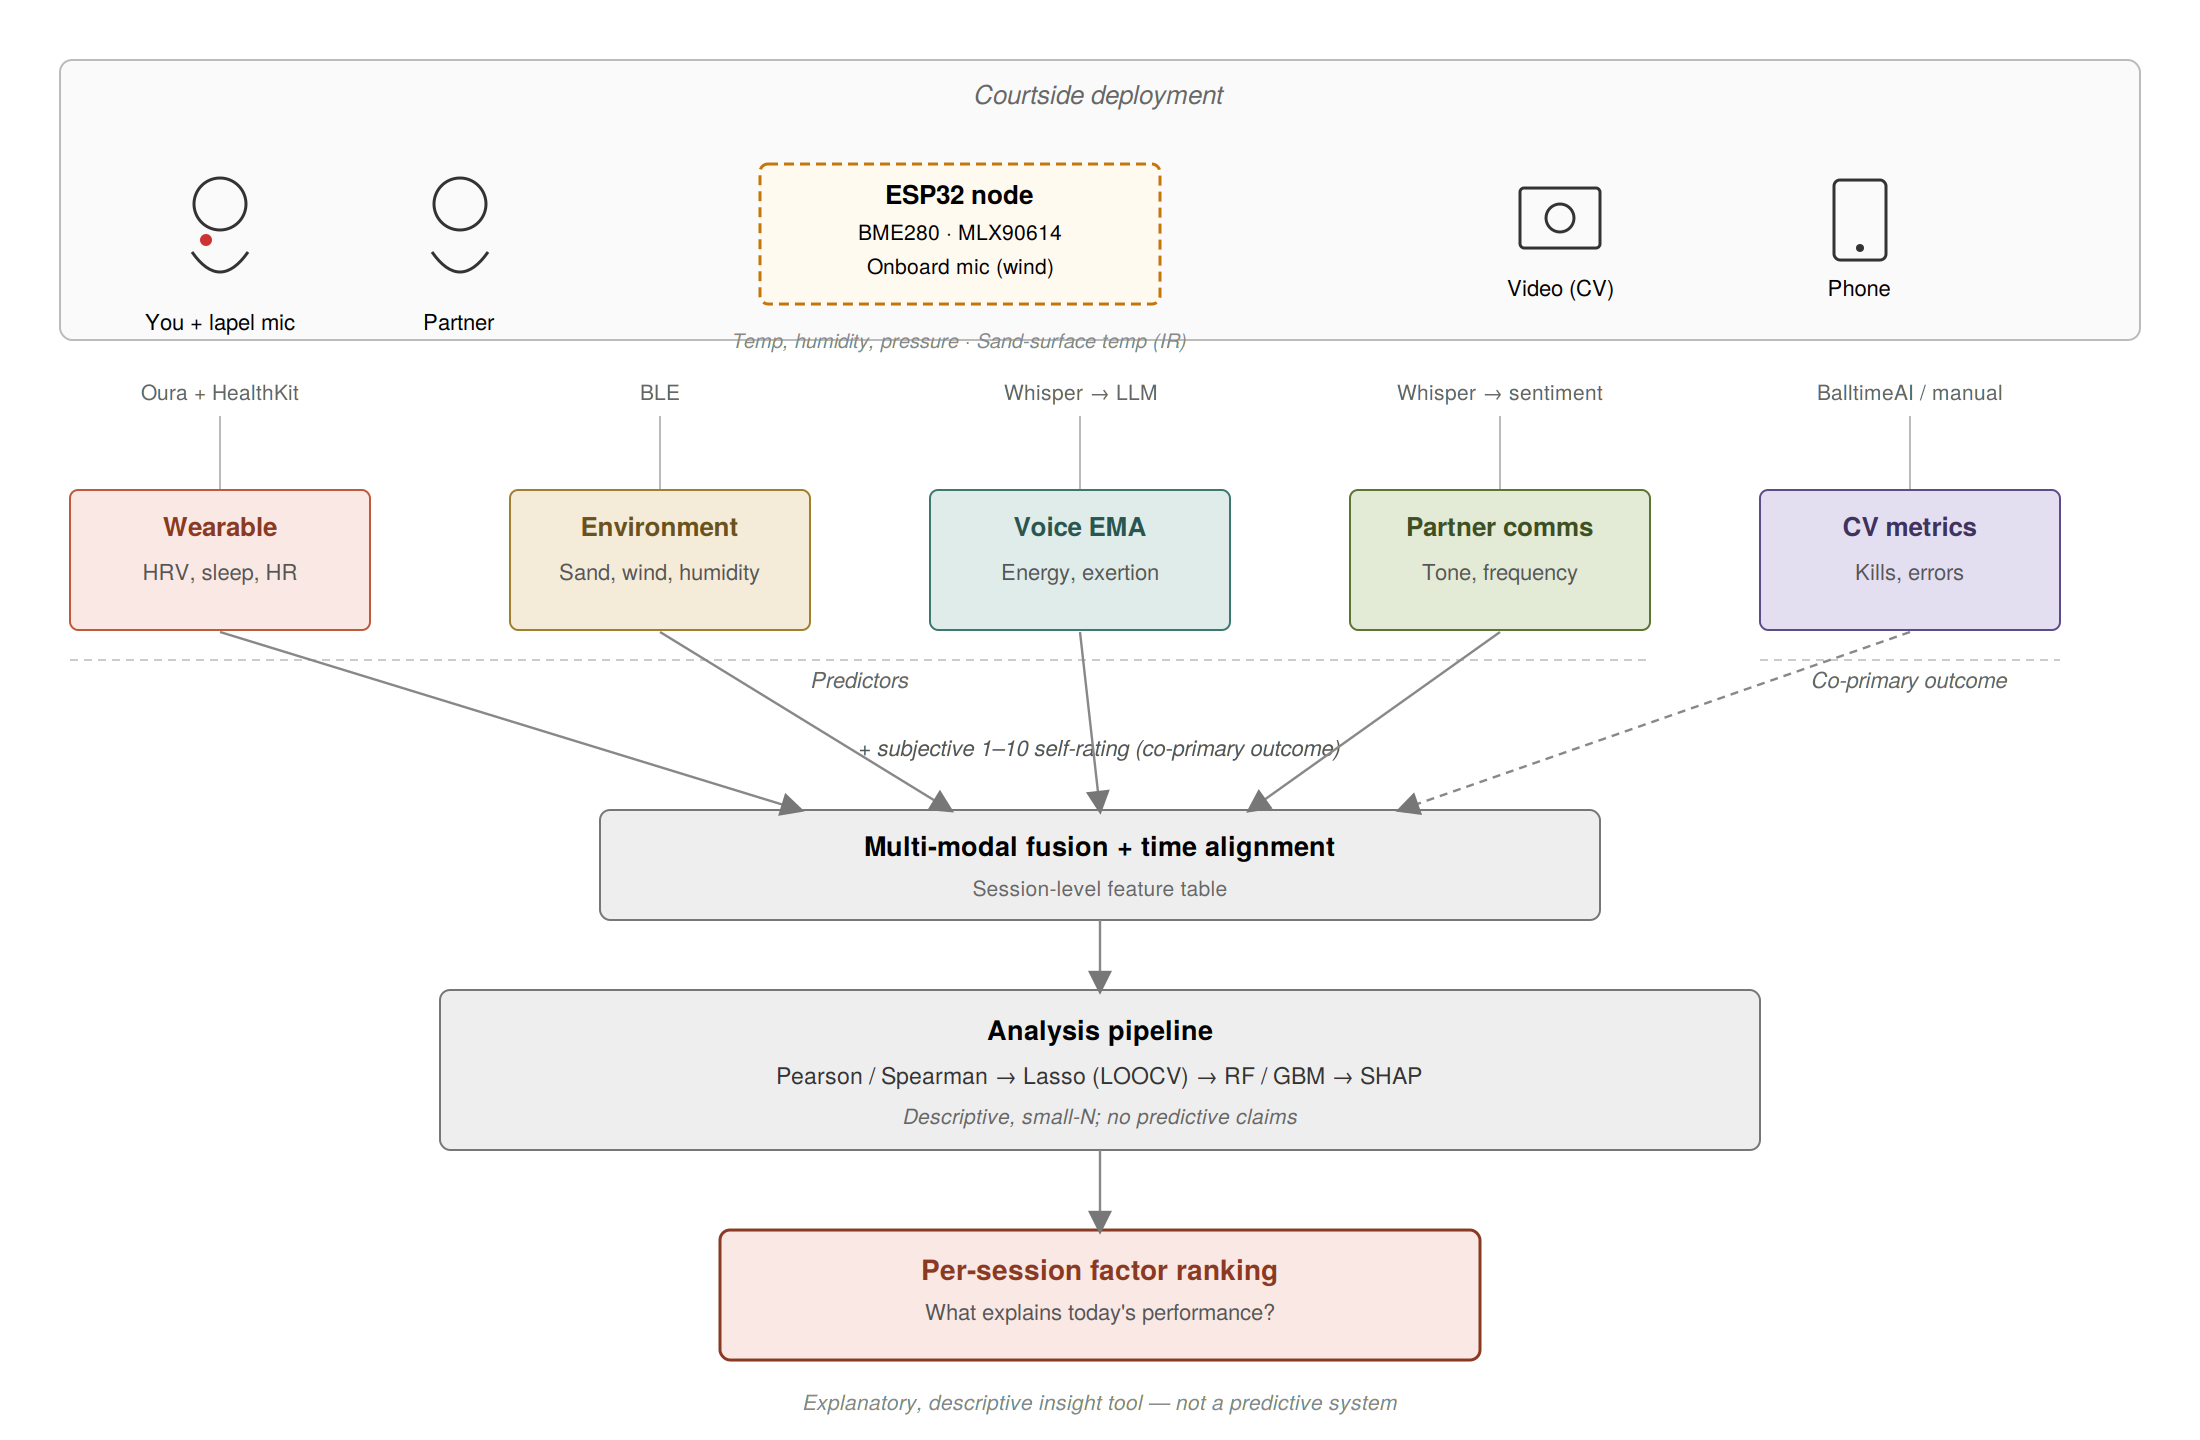
\includegraphics[width=0.9\textwidth]{system_architecture.png}
    \caption{System architecture. The courtside node streams sensor readings over the athlete's phone hotspot to a cloud backend; the Apple Watch and Oura push recovery data to the same backend; the athlete logs subjective/objective outcomes from the mobile web app. All streams are time-aligned into one per-session feature table feeding the four-stage factor-ranking analysis.}
    \label{fig:arch}
\end{figure*}

Figure~\ref{fig:arch} summarizes the deployed end-to-end system; it is a working system, not a mockup.

\subsection{Courtside Environmental Node}
An ESP32-S3 (Fig.~\ref{fig:node}) reads three channels at 1\,Hz: a \textbf{DHT11} (air temperature and humidity, one-wire), an \textbf{MLX90614} non-contact infrared thermometer (sand-surface temperature, I\textsuperscript{2}C address 0x5A; it senses emitted infrared, requiring no contact), and an analog \textbf{electret microphone} whose 50\,ms peak-to-peak amplitude serves as a low-cost wind/audio proxy (on an ADC1 pin so it reads correctly with WiFi active). Firmware connects to the athlete's iPhone Personal Hotspot and HTTP-POSTs each reading as JSON to the backend, with a serial CSV fallback and a boot-time I\textsuperscript{2}C scan for field debugging. The electronics sit in a 3D-printed enclosure with a louvered vent for the air sensor, an open aperture aimed at the sand for the IR sensor (plastic blocks infrared), a foam-screened mic port, and a 1/4-20 tripod mount. The node runs untethered from a USB battery.

\begin{figure}[t]
    \centering
    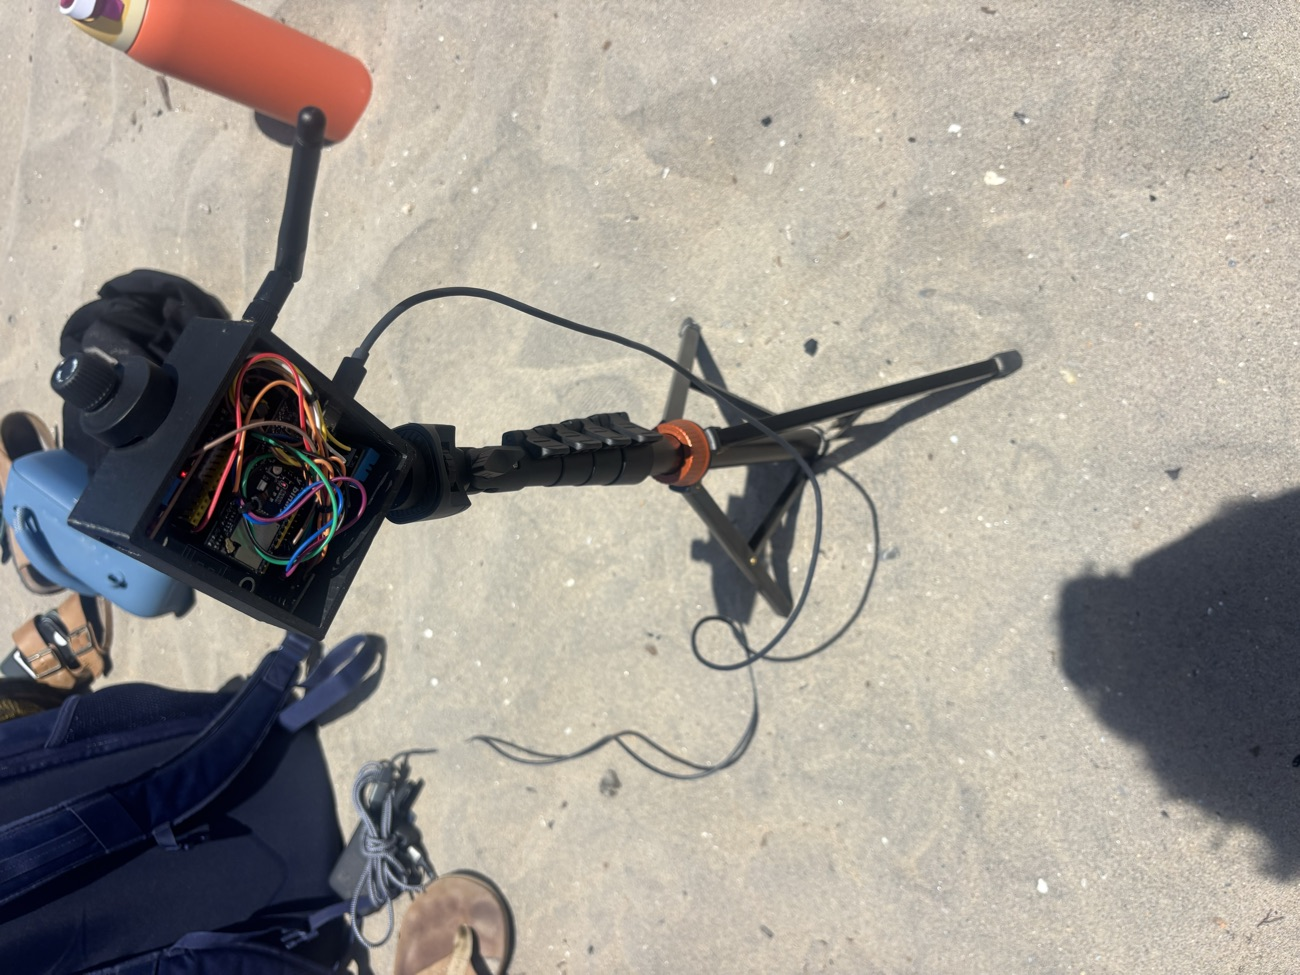
\includegraphics[width=0.6\columnwidth]{node_beach.jpg}\hfill
    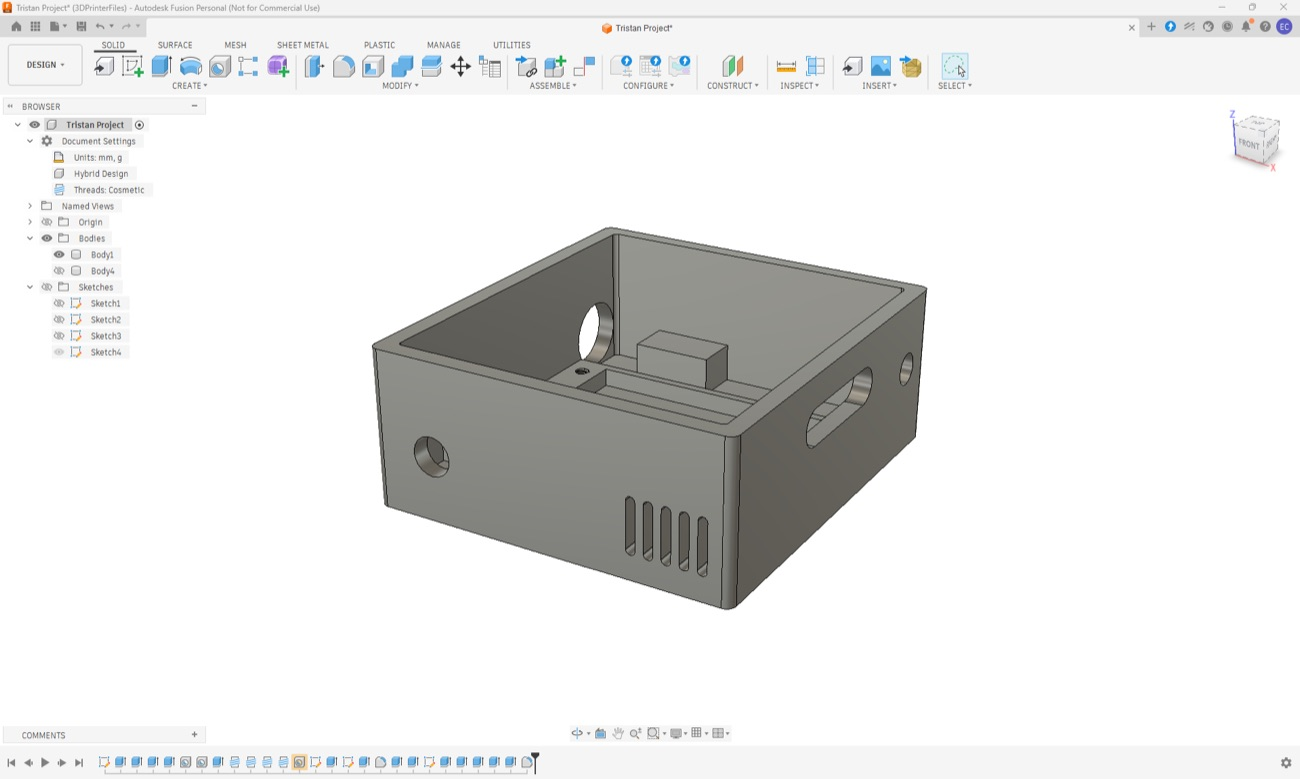
\includegraphics[width=0.37\columnwidth]{enclosure_cad.jpg}
    \caption{Left: the node deployed courtside on sand, tripod-mounted and battery-powered. Right: the enclosure CAD (Fusion~360)---louvered air-sensor vent, open IR aperture, and tripod mount.}
    \label{fig:node}
\end{figure}

\subsection{Cloud Backend and Mobile App}
A FastAPI service with PostgreSQL, deployed on Render, ingests node and wearable data and serves a mobile web app (Fig.~\ref{fig:app}). The app provides: a \emph{live setup view} with real-time per-sensor plots and a heuristic setup-check (e.g., it warns when the IR reading $\approx$ air temperature, indicating the sensor is not aimed at the sand); a \emph{recording} flow that bookmarks each session's start/stop so its sensor time-series window is captured; and an \emph{evaluation} form capturing the subjective 1--10 self-rating, optional peer/coach ratings, felt-wind, kills/errors, partner/opponent, notes, and geolocation. A summary view surfaces recovery, trend, and condition insights.

\begin{figure*}[t]
    \centering
    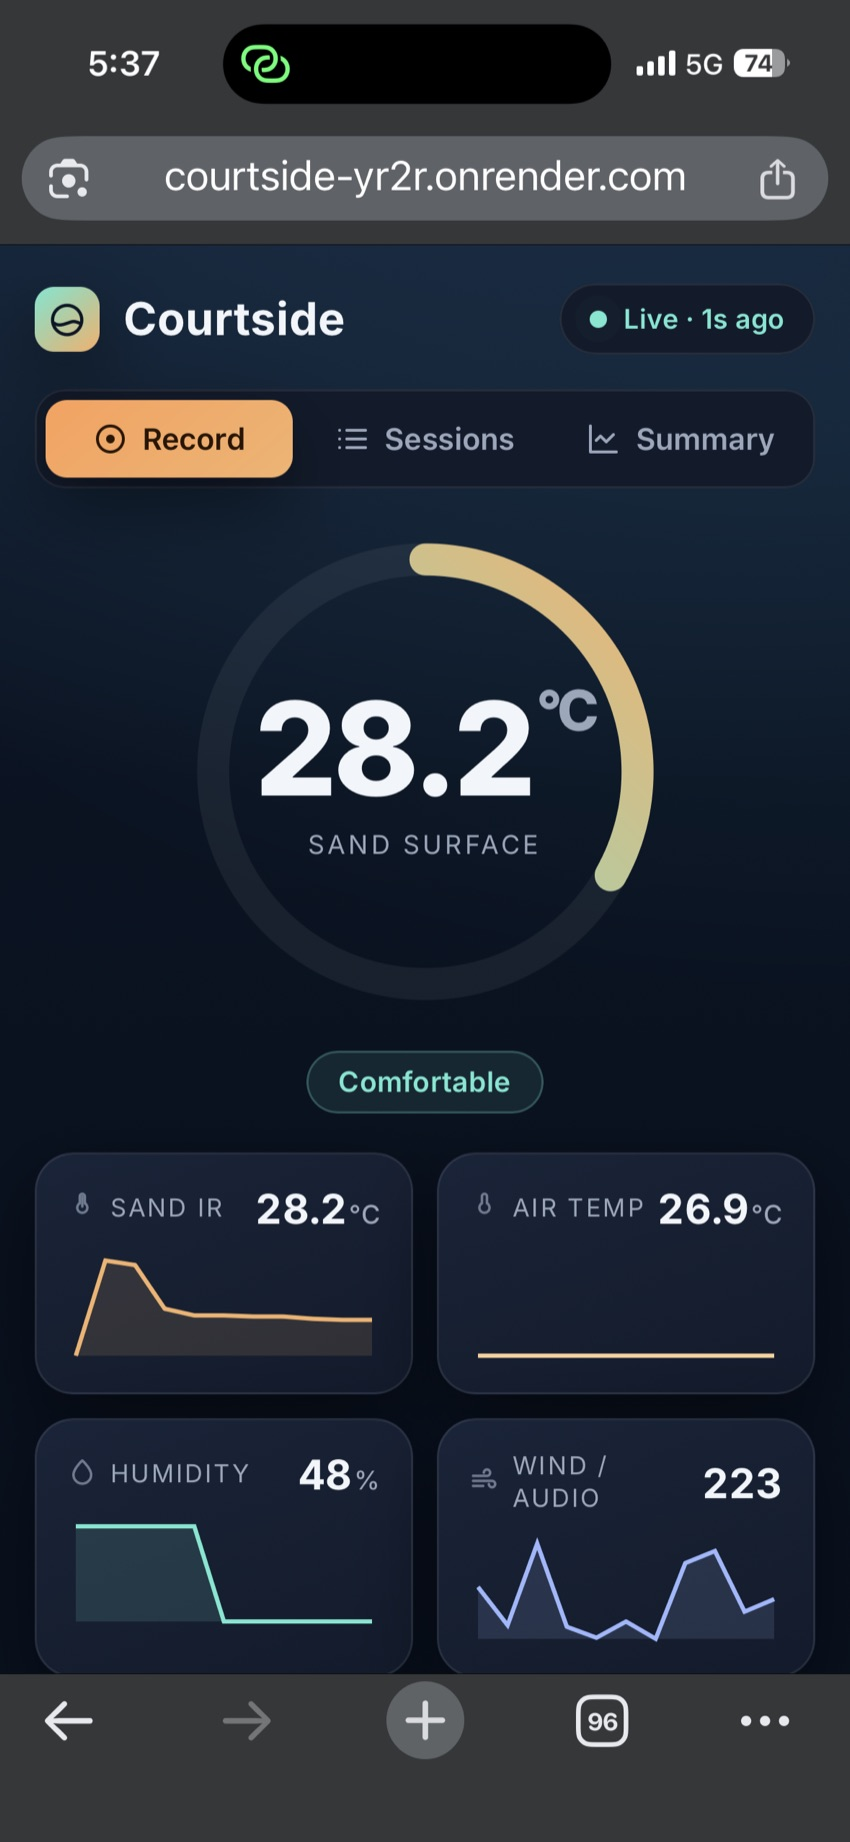
\includegraphics[width=0.31\textwidth]{app_record.jpg}\hfill
    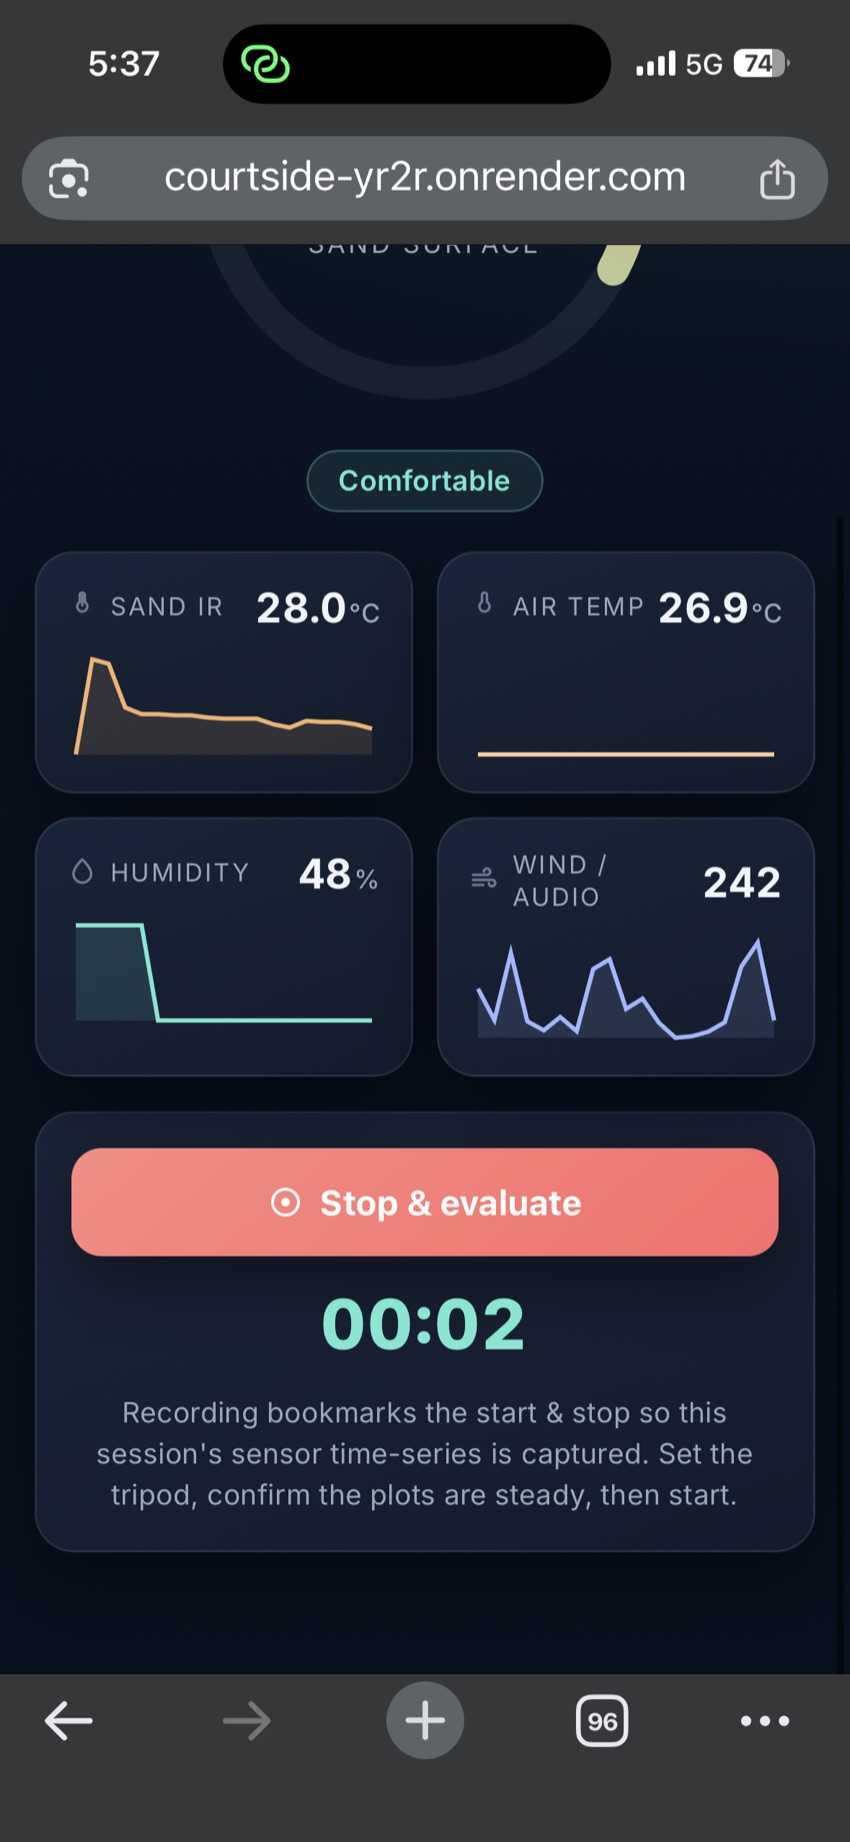
\includegraphics[width=0.31\textwidth]{app_recording.jpg}\hfill
    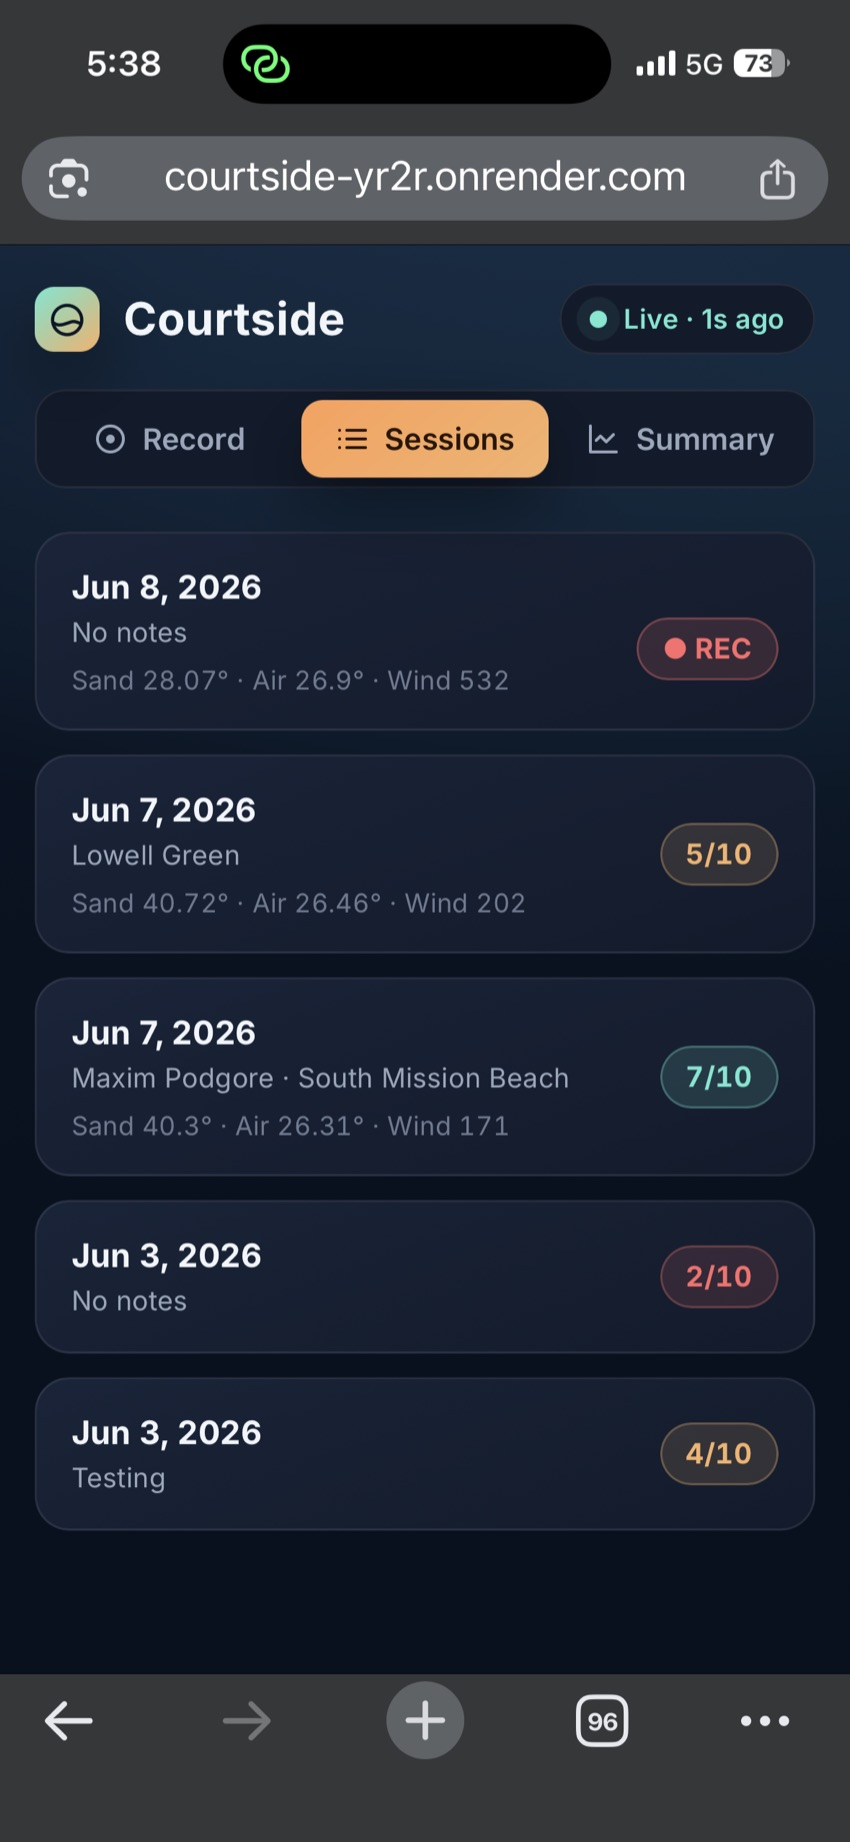
\includegraphics[width=0.31\textwidth]{app_sessions.jpg}
    \caption{The deployed web app on the athlete's phone (live, over cellular). Left: live setup view with the sand-surface ring, per-sensor plots, and a ``Comfortable'' interpretation. Center: an active recording with the elapsed timer. Right: the session list with per-session conditions and value-colored self-ratings (the Jun~7 sessions are real beach data: sand 40.3--40.7\,$^\circ$C).}
    \label{fig:app}
\end{figure*}

\subsection{Wearable and Weather Ingestion}
Apple Watch data syncs automatically via the Health Auto Export app's REST automation, posting HRV (SDNN), resting heart rate, sleep, respiratory rate, and \emph{workouts} to the backend, upserted by date. Every metric is retained losslessly in a raw field so additional signals can be promoted later without re-collection. Oura is pulled via its v2 API as a \emph{second} recovery source, enabling cross-validation (Apple SDNN vs.\ Oura RMSSD). Open-Meteo provides coarse regional weather (wind, gust, temperature, humidity), kept clearly separate from on-court sensor readings as context rather than mixed in.

\subsection{Data Handling and Feature Engineering}
Sensor rows are stamped with server-receive time. Each logged session windows the node readings to its recording interval and aggregates them (mean/max sand and air temperature, mean humidity, mean and 95th-percentile wind-audio). Daily wearable recovery joins by date (Apple preferred, Oura fallback and cross-check). Apple Watch \emph{workouts} overlapping the session window yield in-session intensity (average/max HR, active energy); workouts in the prior seven days yield a cross-training \emph{load} feature. Regional weather is attached per session location. The unit of analysis is the session---appropriate given small $N$---producing one tidy multi-modal feature row per session ($\sim$40 columns).

\subsection{Analysis Pipeline}
The analysis is exploratory and descriptive, in four small-$N$-aware stages: (1) Pearson and Spearman correlations of each feature against the subjective rating; (2) Lasso regression with leave-one-out cross-validation for sparse feature selection; (3) random-forest and gradient-boosting feature importances to capture interactions; (4) SHAP values from the gradient-boosting model for per-factor attribution. We additionally compute leave-one-session-out top-3 stability. The pipeline degrades gracefully: below a sample threshold it emits correlations plus an explicit caveat rather than fabricating a model. No $p$-values are reported as confirmatory, and no model is released for deployment.

\subsection{Evaluation Criteria}
Because the output is a per-session explanation rather than a prediction, standard ML metrics do not apply. We evaluate on engineering criteria: \textbf{data completeness} (fraction of sessions with all streams captured), \textbf{time alignment} (streams aligned to server-receive time and the recording window), \textbf{sensor responsiveness} (bench validation per channel), and \textbf{ranking stability / face validity} (leave-one-session-out stability and comparison of top factors to the athlete's recollection)---the latter two meaningful only once $N$ is sufficient.

%===================================================================
\section{Results}
%===================================================================
\subsection{User-Need Validation (N=20)}
Before further hardware investment we surveyed 20 players (UCSD men's/women's beach teams plus recreational, club, NCAA, and Open/AVP players) to validate need and prioritize features (Fig.~\ref{fig:survey}). \textbf{Wind ranked first} (4.05/5), validating the decision to prioritize wind sensing; recovery/tiredness, mental state, partner identity, and partner communication completed the top five; court noise, location, and pace of play ranked lowest and were dropped from the feature plan. Open responses repeatedly raised \emph{food timing}, \emph{soreness}, and \emph{warm-up quality}, motivating lightweight subjective inputs. Across the cohort, 85\% expressed positive interest, with qualified interest centered on wearable integration and minimal in-session burden.

\begin{figure}[t]
    \centering
    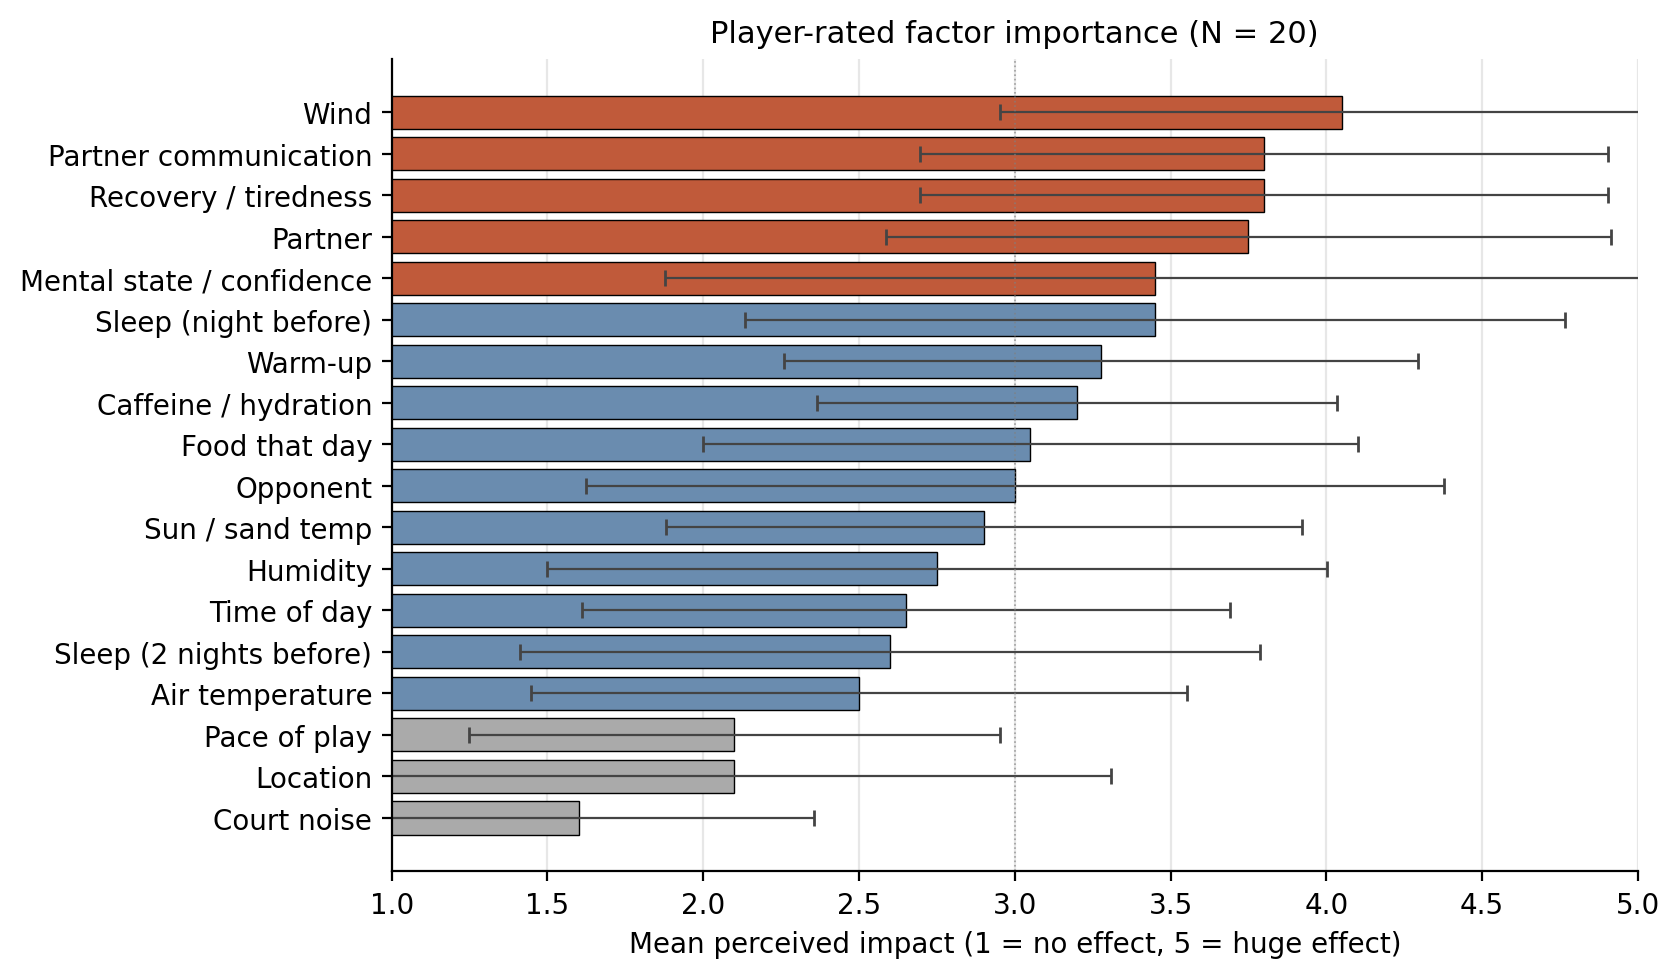
\includegraphics[width=0.97\columnwidth]{factor_rankings.png}
    \caption{Player-rated factor importance ($N=20$), mean $\pm$ 1 SD. Wind ranks first overall. Top five (orange) retained as primary engineered features; bottom three (gray) dropped.}
    \label{fig:survey}
\end{figure}

\subsection{Sensor Validation (Bench)}
Each channel was validated for responsiveness (Fig.~\ref{fig:bench}): exhaling on the node produces the expected coupled DHT11 temperature/humidity spike with exponential return to ambient; blowing across the microphone produces clear transient amplitude spikes above a stable baseline; and the MLX90614 tracks a warm surface in its field of view (an immediate $\sim$10\,$^\circ$C rise aimed at skin). The Oura API pipeline was separately validated against a 21-day rolling window.

\begin{figure}[t]
    \centering
    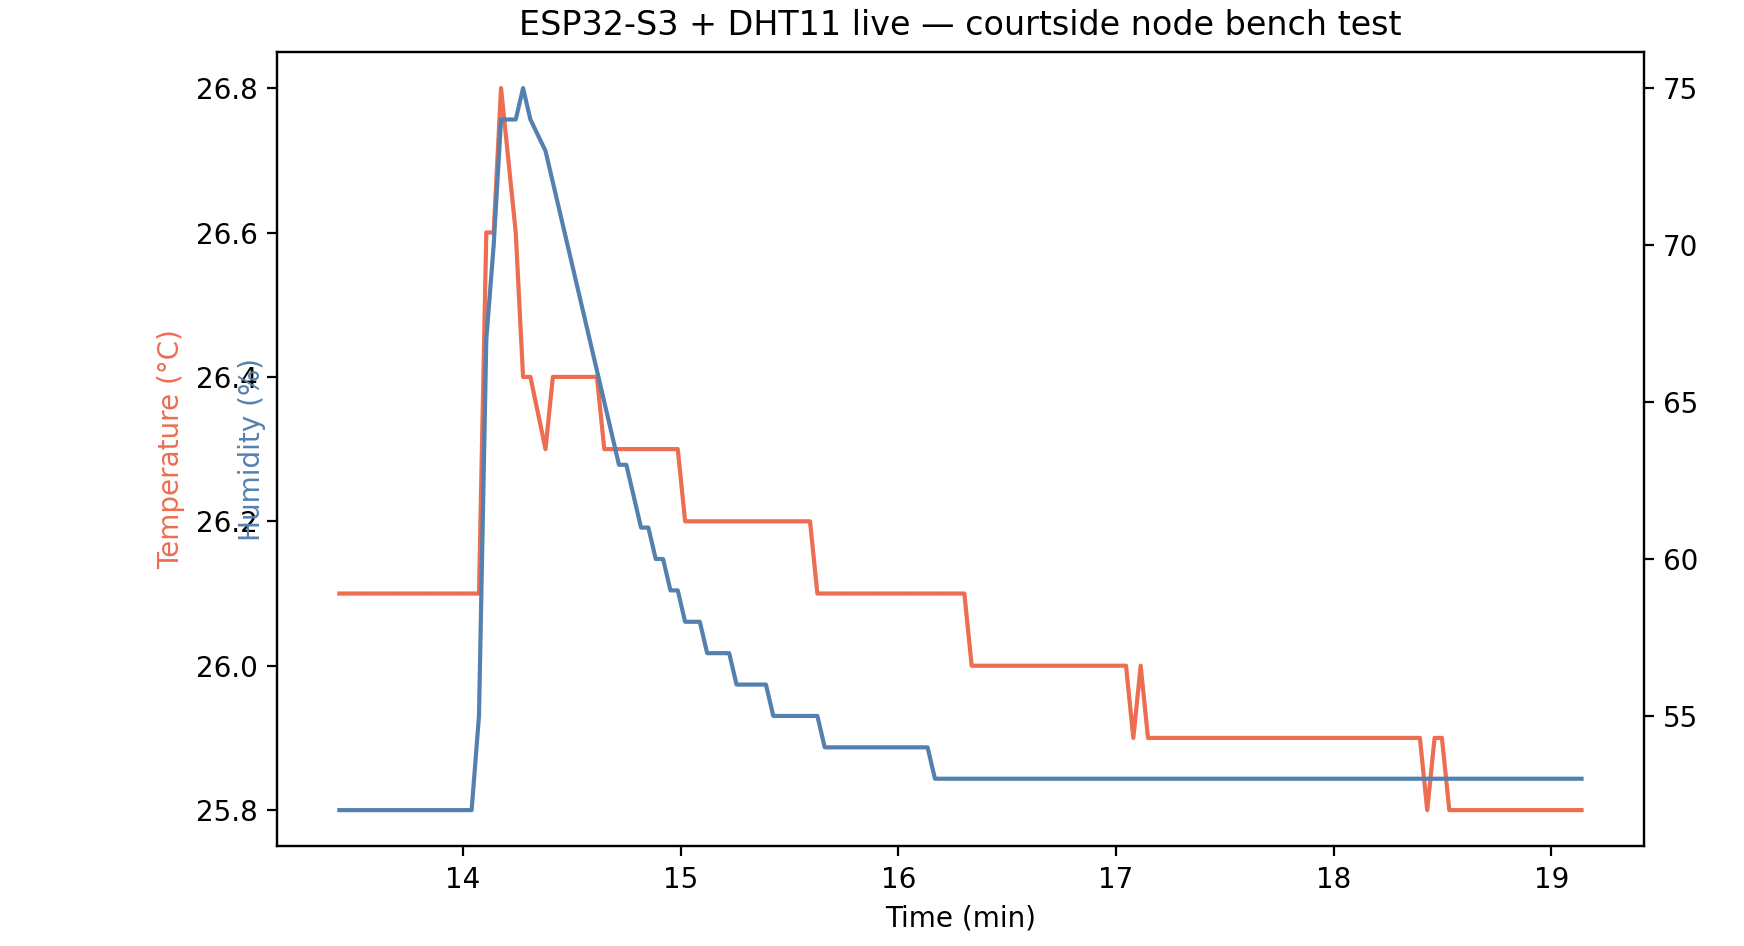
\includegraphics[width=0.49\columnwidth]{esp32_bench.png}\hfill
    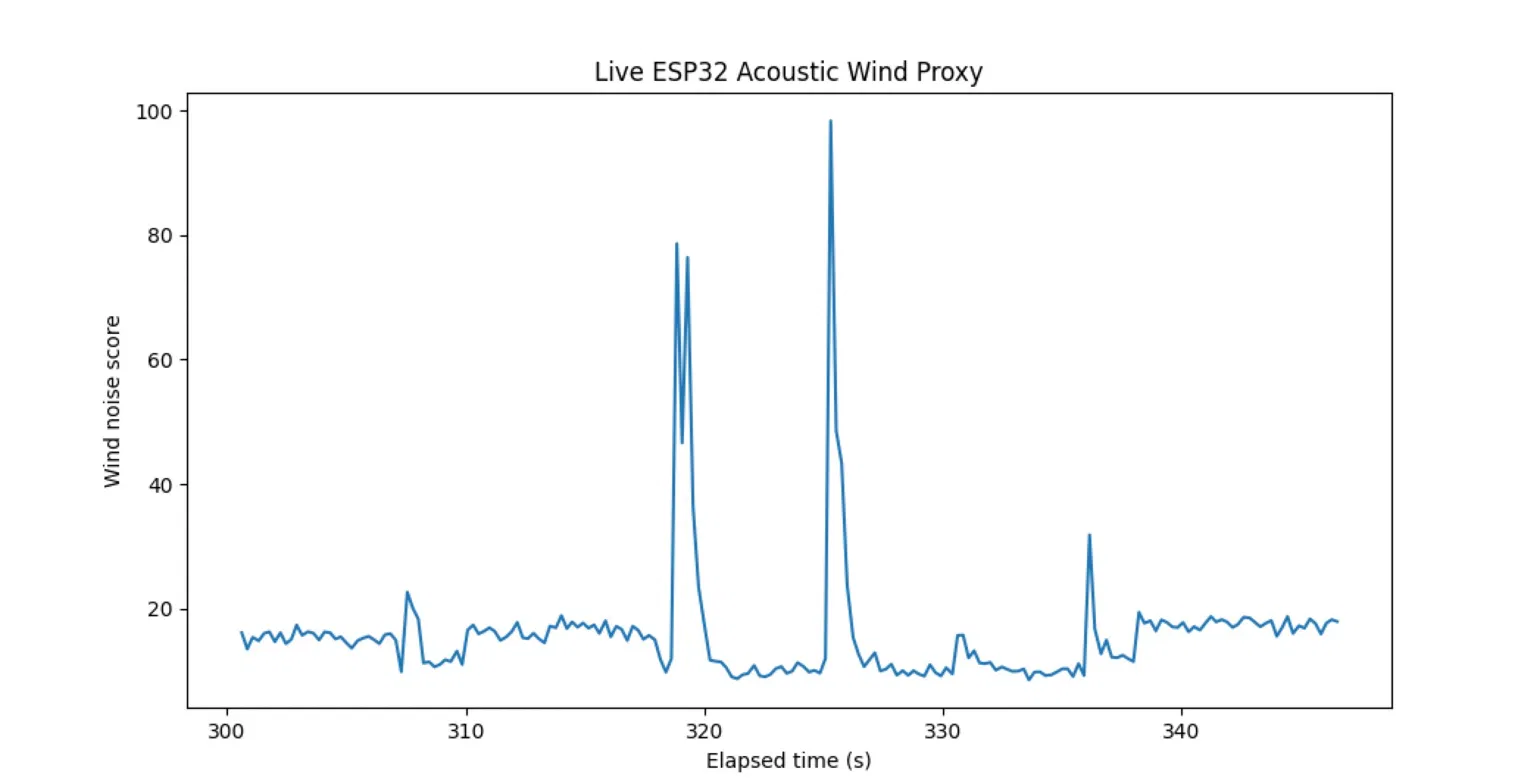
\includegraphics[width=0.49\columnwidth]{wind_proxy.png}
    \caption{Bench validation. Left: an exhalation event ($t\approx14$~min) produces a coupled temperature/humidity response. Right: the acoustic wind proxy responds to blown-air transients above a stable baseline.}
    \label{fig:bench}
\end{figure}

\subsection{Live Courtside Pilot}
The full wireless path was exercised on the beach: the node ran from a USB battery, joined the phone hotspot, and streamed to the cloud while the athlete used the live dashboard to position the tripod. On the first instrumented day we recorded two sessions of $\sim$1{,}380 and $\sim$2{,}255 one-Hz samples, with sand-surface temperatures of \textbf{40--43\,$^\circ$C} against $\sim$26\,$^\circ$C air---directly demonstrating the court-level microclimate weather data cannot capture. Apple Watch recovery for the same window arrived automatically (HRV, resting HR, sleep), and three Volleyball workouts were ingested with in-session heart rate (average 140--172\,bpm, peak 174--186\,bpm) and active energy (160--459\,kcal). The build step assembled a $\sim$40-column multi-modal feature row per session, confirming end-to-end fusion.

\subsection{Pipeline Demonstration (Simulated)}
Because real $N$ is currently too small for interpretable ranking (a four-point correlation can exceed 0.8 by chance), we ran the unmodified pipeline on a \emph{clearly labeled simulated} dataset of 16 sessions with a planted plausible structure (better sleep/HRV and cooler, calmer conditions $\rightarrow$ higher rating). The pipeline recovers that structure (Fig.~\ref{fig:sim}): HRV correlates positively ($r\approx0.67$) and sand-surface temperature negatively ($r\approx-0.36$) with the rating, and the leave-one-session-out stability column flags which factors are robust. This is shown to demonstrate \emph{what the instrument produces at scale}, not as a finding.

\begin{figure}[t]
    \centering
    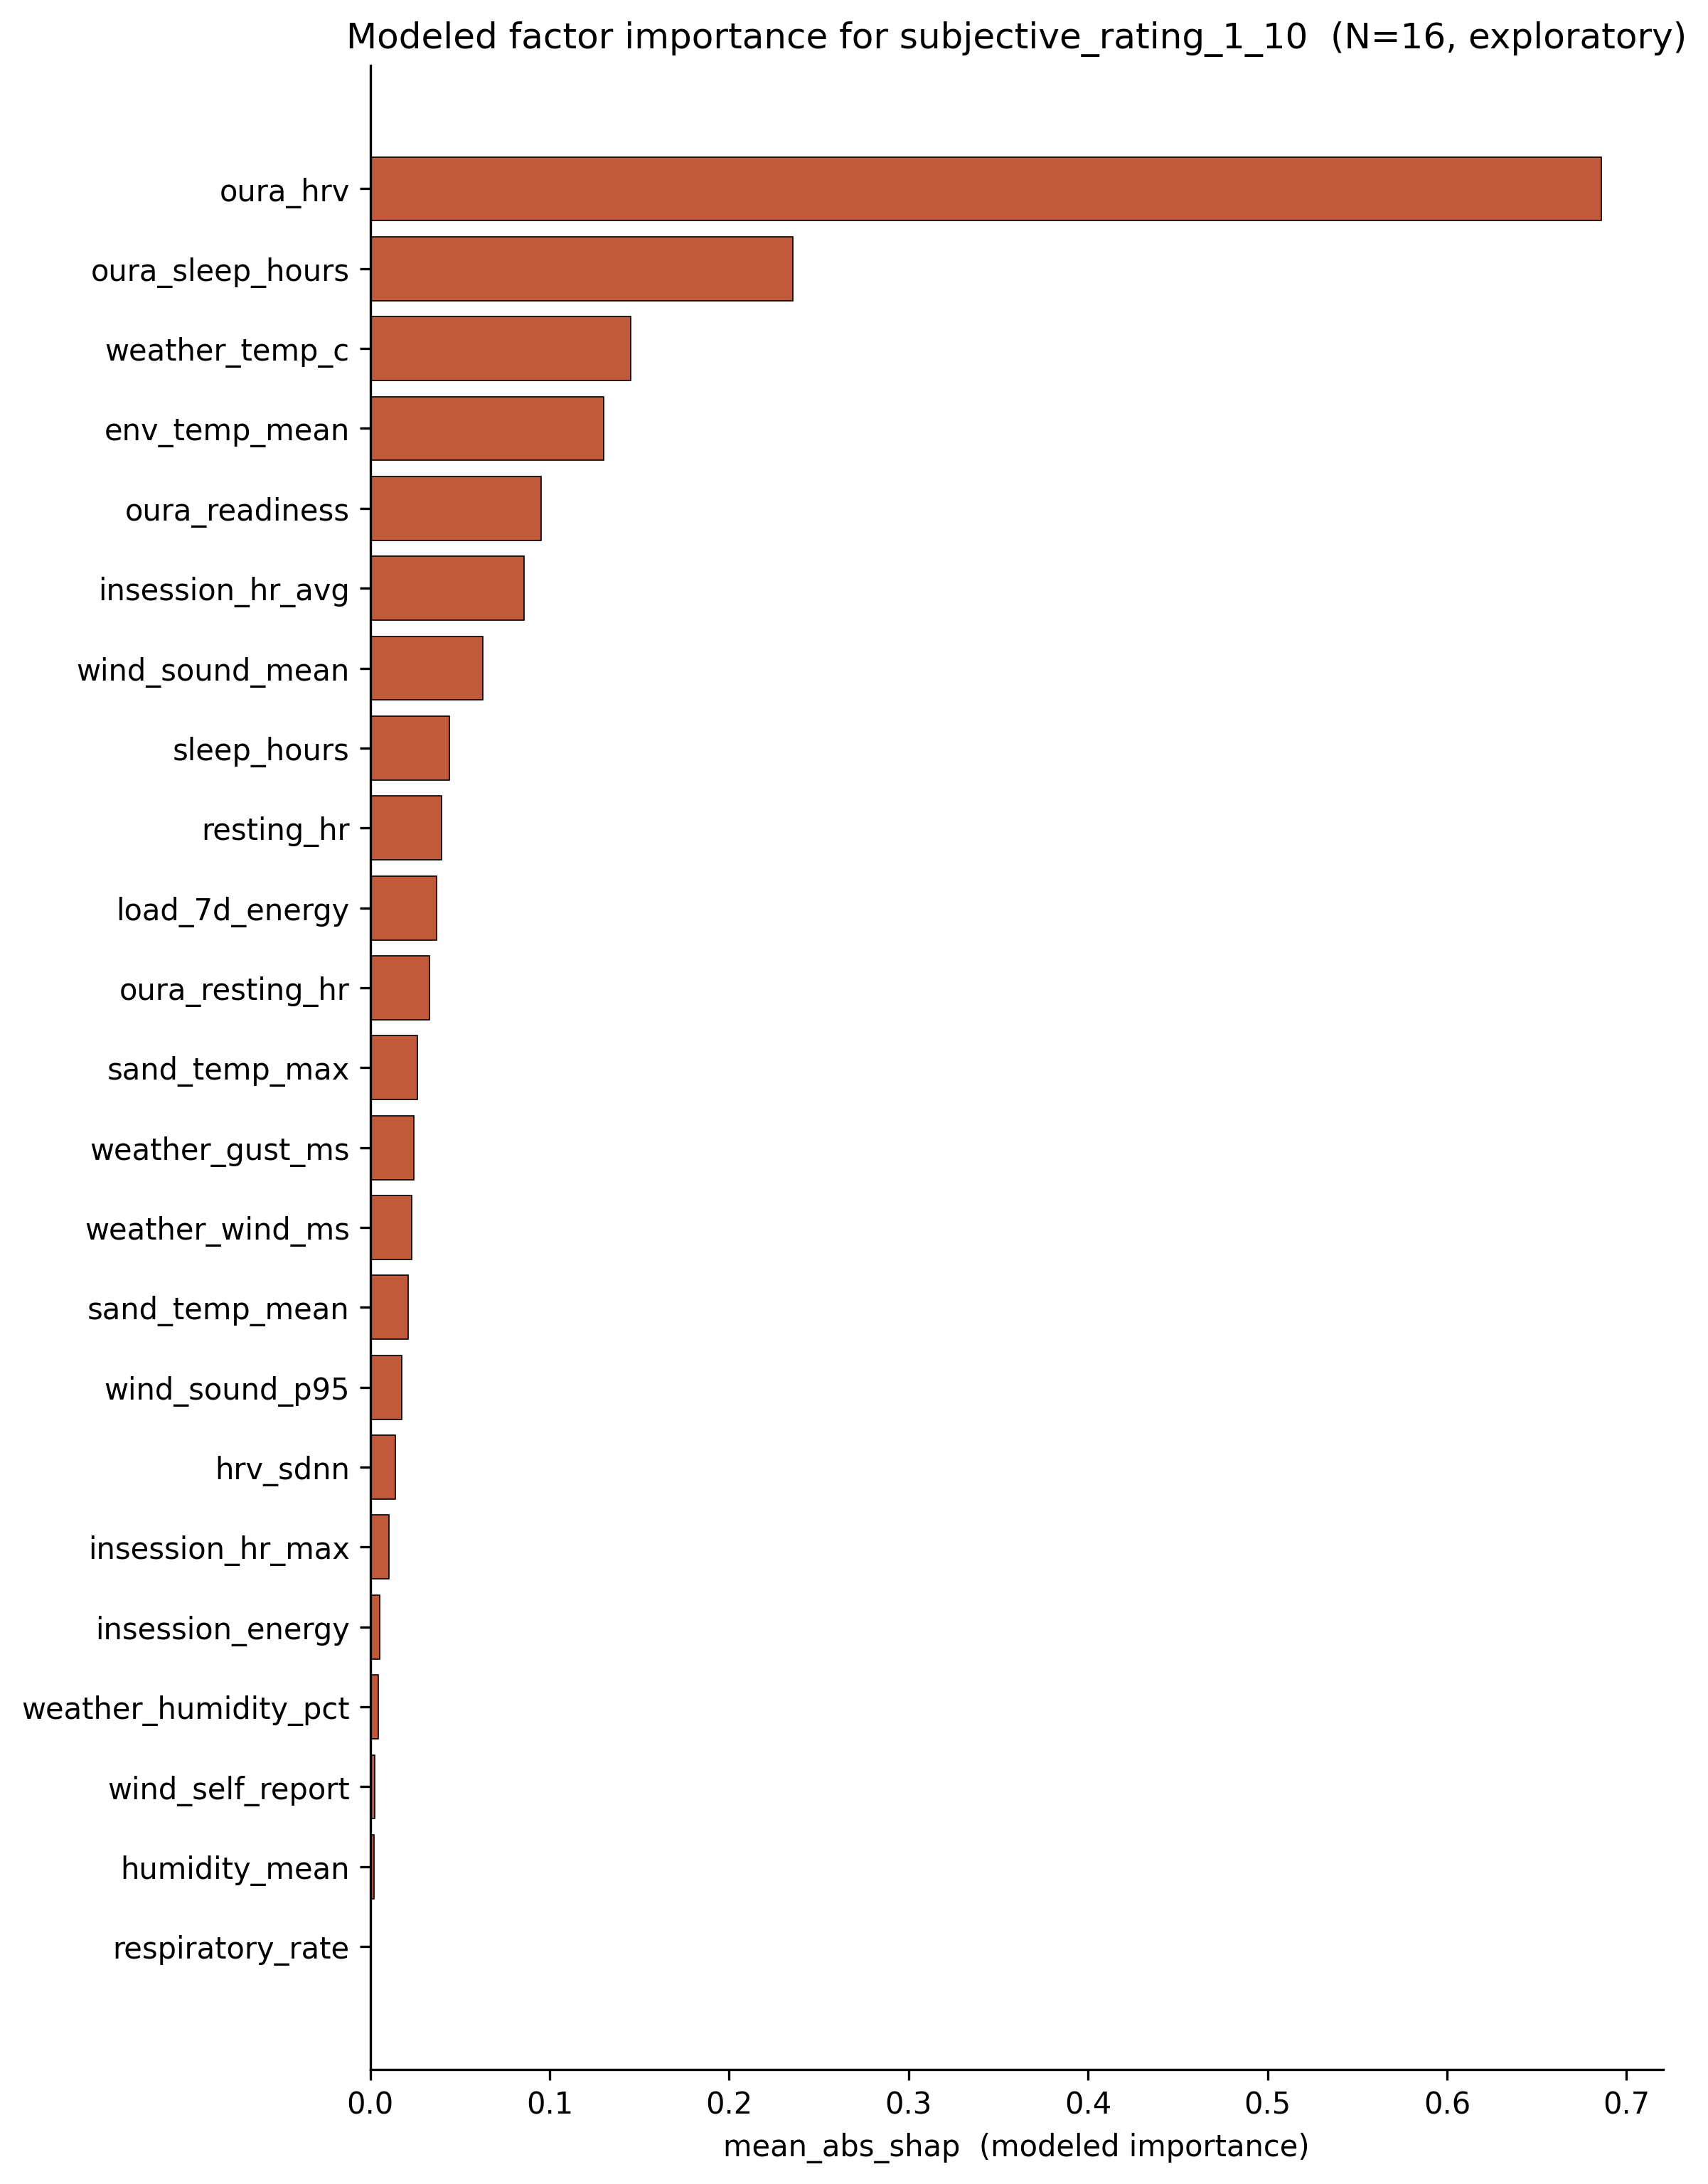
\includegraphics[width=0.97\columnwidth]{factor_rankings_sim.png}
    \caption{Pipeline factor-ranking \emph{output} on a labeled \textbf{simulated} 16-session dataset (not real data). Demonstrates the end-to-end analysis and its self-reported stability. Real-data ranking awaits sufficient $N$.}
    \label{fig:sim}
\end{figure}

The instrument also supports targeted, personally-actionable relationship views (Fig.~\ref{fig:rel}). Pairing each Apple Watch workout to its ESP32 session window by \emph{timestamp overlap} yields \emph{actual effort} (in-session heart rate) alongside \emph{reported performance}; overnight \emph{sleep} can likewise be plotted against performance. On the simulated data, sleep tracks self-rated performance strongly ($r\approx0.83$) while raw physical effort does not ($r\approx0.27$)---exactly the kind of contrast the tool is designed to surface, and a reminder that more effort is not more performance.

\begin{figure}[t]
    \centering
    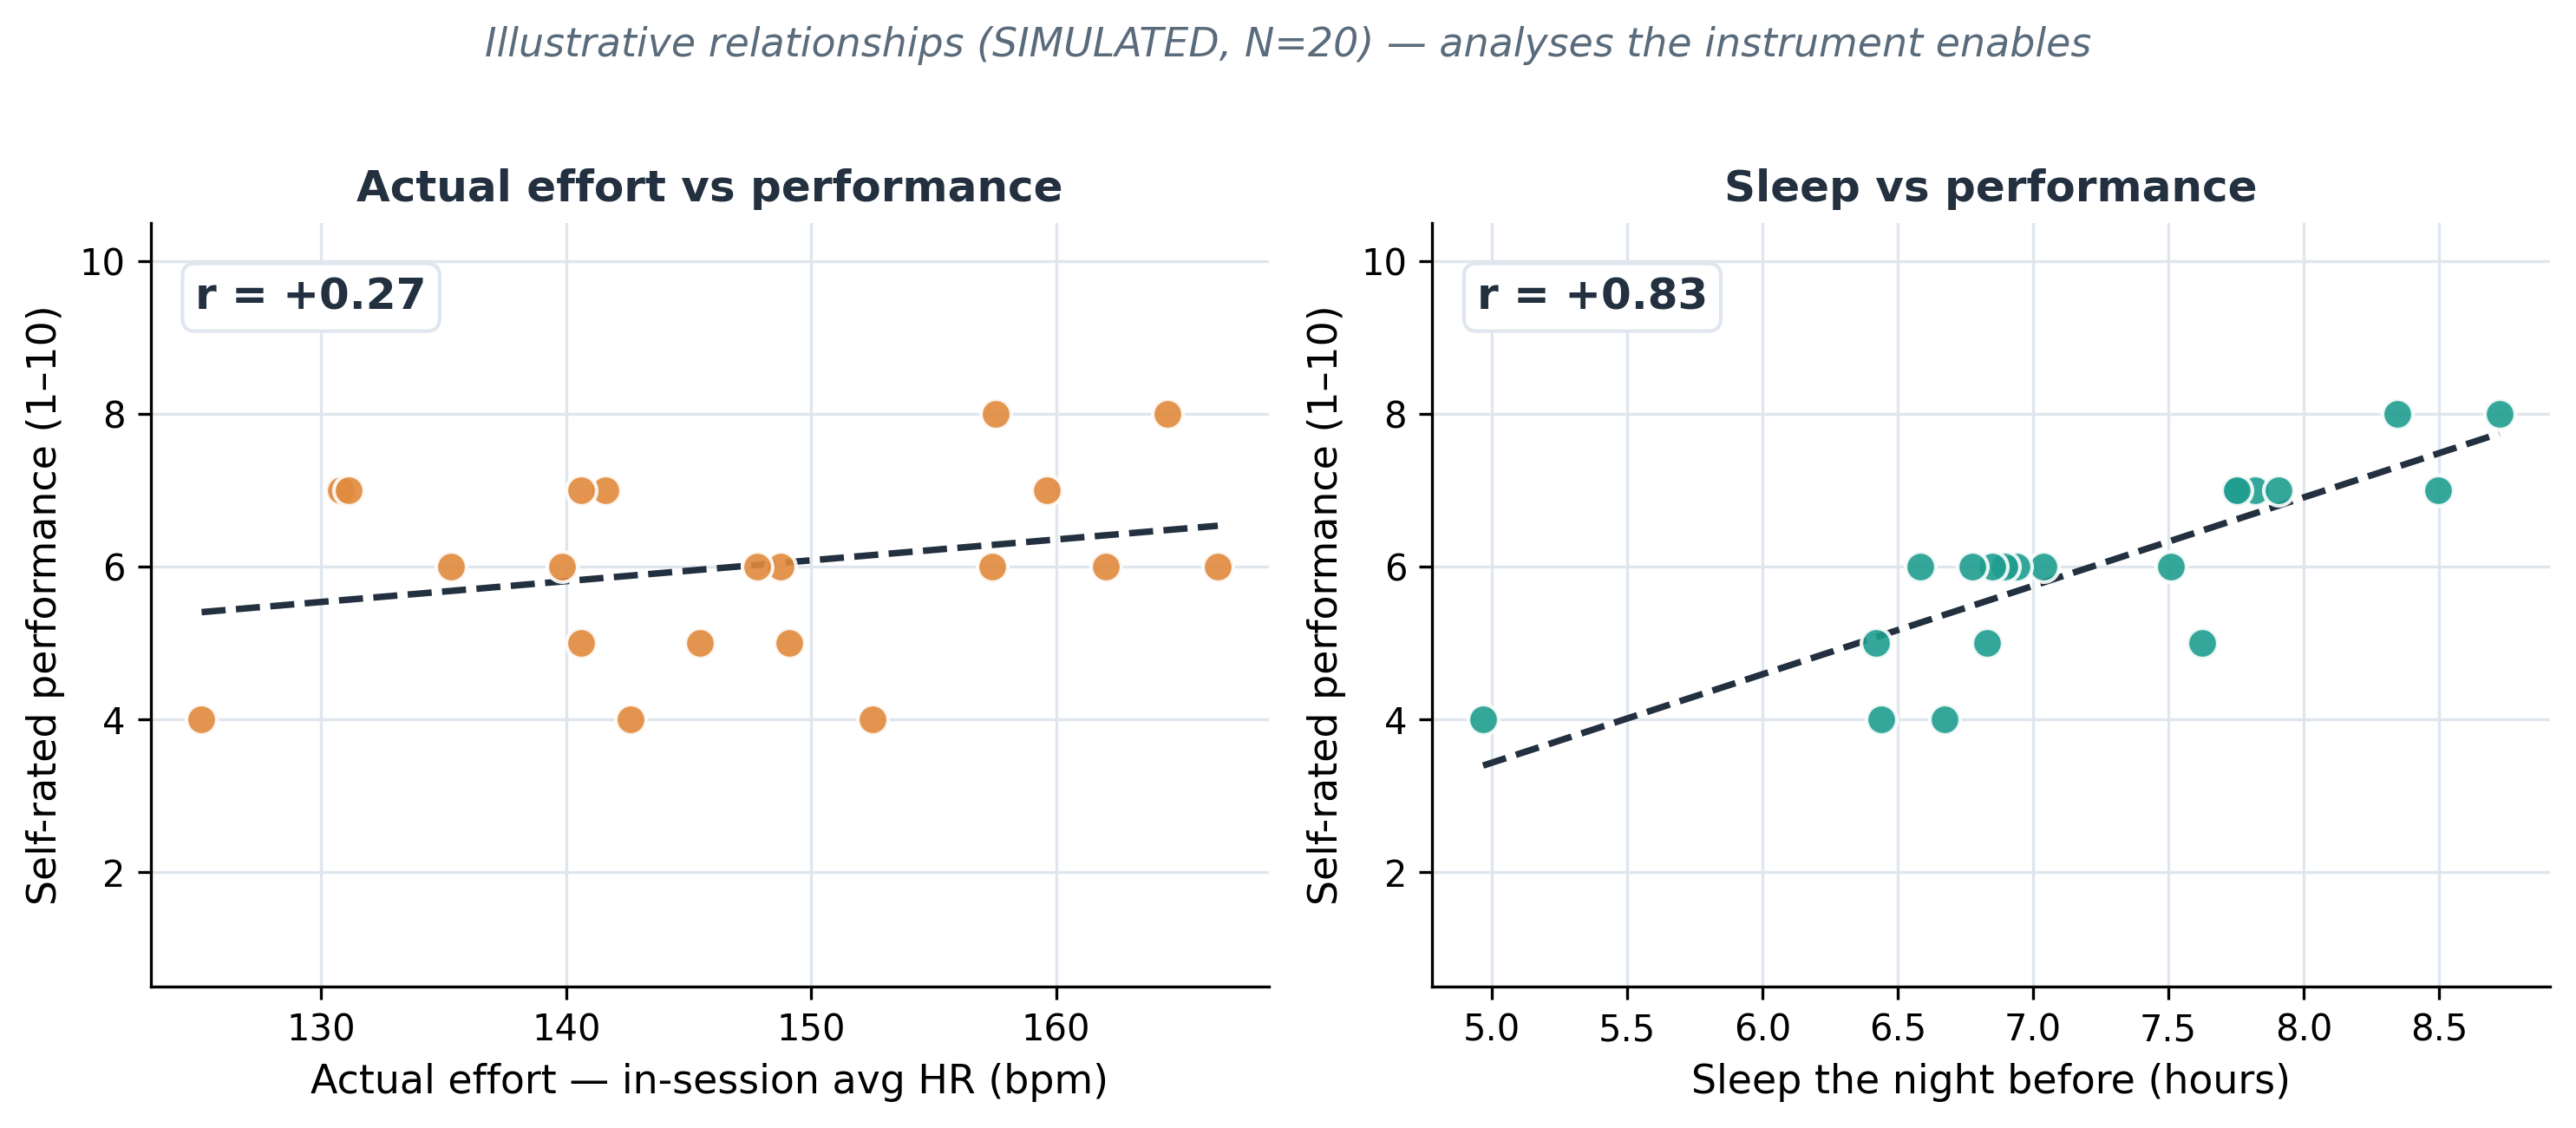
\includegraphics[width=0.99\columnwidth]{demo_relationships.png}
    \caption{Illustrative (\textbf{simulated}) relationship views the instrument produces from paired streams: actual effort (watch in-session HR, timestamp-matched to the ESP32 session) vs.\ self-rated performance (left), and sleep vs.\ performance (right). Shown to illustrate the analysis; not a real-data finding.}
    \label{fig:rel}
\end{figure}

%===================================================================
\section{Discussion}
\label{sec:discussion}
%===================================================================
\textbf{What worked.} The hardest integration risks---untethered wireless streaming from a beach, automated wearable ingestion, and time-aligned multi-modal fusion---are all working and deployed. The court-level microclimate signal (40\,$^\circ$C+ sand vs.\ 26\,$^\circ$C air) is real and is precisely the value a single wearable or weather app misses.

\textbf{Honest limitations.} \emph{Small $N$ is the dominant limitation}: factor rankings on a handful of real sessions are not statistically interpretable, so all real output is framed descriptively and the pipeline reports its own instability. \emph{Ground truth:} the subjective 1--10 rating is the primary outcome; kills/errors are secondary and heavily confounded by partner and opponent in 2v2 play, so we added optional \emph{peer and coach ratings} as higher-quality external truth and reserve per-own-contact statistics for future work. \emph{Sensor fidelity:} the DHT11 is low-resolution ($\pm$2\,$^\circ$C, $\pm$5\%\,RH; no barometric pressure, hence the BME280 substitution); the microphone is an uncalibrated qualitative wind proxy, validated against self-reported wind and regional weather rather than an anemometer; regional weather is $\sim$1--3\,km grid-scale by design. \emph{Scope:} voice EMA and CV kill/error extraction were de-scoped to keep the core robust.

\textbf{Reviewer feedback addressed.} Per TA and classmate feedback: the report is tightened for length and uses judicious figures; the survey is elevated as user-need validation; the kills/errors confound is reframed with peer/coach ground truth added; figures are exported at high resolution; an evaluation section reports what is measurable at current $N$ plus a concrete plan; the analysis is a committed four-stage pipeline with specified per-stream data handling.

\textbf{Generalization.} The patterns---time-aligning heterogeneous low-cost streams, capturing microclimate that regional data misses, small-$N$ feature ranking with honest stability reporting, and face-validity evaluation---transfer to other outdoor, individually-variable, heat-exposed settings (e.g., heat-exposed workers).

%===================================================================
\section{Conclusion}
%===================================================================
We delivered a working, deployed multi-modal instrument and analysis pipeline that fuses court-level environmental sensing, wearable recovery and in-session intensity, regional weather, and subjective performance for an individual beach volleyball athlete, grounded in a 20-player needs survey and validated end-to-end on a live beach pilot. The main takeaway: the integration is real and the court microclimate it captures is genuinely invisible to existing tools; the honest gap is sample size, and because the instrument now collects all streams at near-zero marginal effort, the remaining work---reaching $\geq$15 sessions and re-running the already-built ranking---is straightforward. We present simulated output to show what the system produces at scale, and we make no statistical claims on the small real sample.

\section*{AI Use Disclosure}
AI tools (Claude) were used as a pair-programming and drafting assistant for the firmware, backend, and web-app code, for editing this report's prose, and to summarize open-ended survey responses. All system design, hardware integration, data-collection methodology, analysis choices, and the underlying data are the author's own. No AI tools were used during oral assessments.

\end{document}
